\chapter{Τίτλος κεφαλαίου}
\label{chap2}

\section{Εισαγωγή}
Τα δυναμικά προγράμματα τιμολόγησης παρουσιάζουν όλο και μεγαλύτερο ενδιαφέρον από δημόσιες κρατικές επιτροπές και επιχειρήσεις κοινής ωφέλειας ενώ οι βιομηχανίες συνεχίζουν το σχεδιασμό για τη δημιουργία των έξυπνων δικτύων. Αυτό συμβαίνει γιατί οι επιχειρήσεις κοινής ωφέλειας ανά τον κόσμο δεν επιτρέπουν την αμφίδρομη σχέση με τον καταναλωτή ώστε να μπορεί να είναι ο ίδιος ρυθμιστής της κατανάλωσης ενέργειας ανάλογα με τις ανάγκες του.

Μελέτες διαφόρων ερευνητικών ομάδων έδειξαν ότι το κόστος δεν κατανέμεται ισομερώς. Οι καταναλωτές οι οποίοι βρίσκονται υπό καθεστώς <<επίπεδης>> τιμολόγησης κατανάλωσαν περισσότερη ενέργεια κατά τις ώρες αιχμής. Με τα δυναμικά προγράμματα τιμολόγησης υπάρχει η δυνατότητα να επιλυθεί αυτό το πρόβλημα με την ενίσχυση της οικονομικής αποδοτικότητας έχοντας σαν αποτέλεσμα την μείωση της ζήτησης σε ώρες αιχμής.

\section{Ορισμός Δυναμικής Τιμολόγησης}
Με τον όρο Δυναμική Τιμολόγηση (dynamic pricing) εννοούμε την δυνατότητα που δίνει ο πάροχος στον πελάτη του, να τιμολογείται με μία τιμή που διαφέρει από ώρα σε ώρα, ενώ για κάθε 24ωρο οι τιμές ανακοινώνονται, οι τιμές ανακοινώνονται από μια μέρα έως και λίγες ώρες πριν. Για τον υπολογισμό αυτής λαμβάνεται υπόψη η τιμή στη χονδρική αγορά, το κόστος για την χρήση των δικτύων, το κέρδος του παρόχου και άλλες χρεώσεις. Με αυτό τον τρόπο οι καταναλωτές εκτίθενται στο ρίσκο της τιμής που διαμορφώνεται ανά ώρα αλλά γλιτώνουν τη χρέωση που θα τους επέβαλε ο πάροχός τους, εάν αναλάμβανε εκείνος να διαχειριστεί το ρίσκο αυτό. Με την μετάβαση σε δυναμικά τιμολόγια αναμένεται ότι κάποιοι καταναλωτές θα ωφεληθούν ενώ κάποιοι άλλοι θα χάσουν. Εκείνοι οι οποίοι θα χάσουν είναι αυτοί που πραγματοποιούν τη μεγαλύτερη κατανάλωση ενέργειας σε ώρες αιχμής. Αντίθετα, εκείνοι οι οποίοι θα κερδίσουν είναι αυτοί που παρουσιάζουν τη λεγόμενη "επίπεδη" κατανάλωση δηλαδή δεν καταναλώνουν μεγάλη ποσότητα ενέργειας σε ώρες αιχμής. Υπάρχουν και αυτοί οι οποίοι δεν έχουν ούτε όφελος ούτε ζημία γιατί το προφίλ κατανάλωσης ταυτίζεται με τη καμπύλη φορτίου (και κόστους) του συστήματος (υποθέτουμε ανασχεδιασμό τιμολογίων ουδέτερο ως προς τα συνολικά έσοδα του προμηθευτή)~\cite{[MR99]}.

\section{Μεταβαλλόμενη τιμή της ενέργειας}
Επειδή υπάρχει μεγάλη αδυναμία των πελατών της λιανικής αγοράς και των φορτίων τους να συμμετέχουν στις αγορές, οι σύγχρονες ηλεκτρικής ενέργειας δεν είναι αρκετά αποτελεσματικές όσον αφορά τον ανταγωνισμό. Η τιμή της ηλεκτρικής ενέργειας στην αγορά μεταβάλλεται από ώρα σε ώρα συχνά ακόμα και κατά 30-50\% μέσα σε μια μέρα. Οι λόγοι για τους οποίους η τιμή της ηλεκτρικής ενέργειας παρουσιάζει αυτή τη συμπεριφορά είναι οι εξής~\cite{[R85],[G95]}:
\begin{enumerate}
\item	Το κόστος της ηλεκτρικής ενέργειας διαφέρει πολλές φορές ανάλογα με την τεχνολογία που χρησιμοποιείται.(Για παράδειγμα οι υδροηλεκτρικές μονάδες και εκείνες που χρησιμοποιούν την πυρηνική ενέργεια έχουν κόστος κάτω των 10\$/ΜWh, ενώ το κόστος για μια συμβατική μονάδα ορυκτών καυσίμων ανέρχεται περίπου στα 100\$/MWh).
\item	Το φορτίο του συστήματος μεταβάλλεται από ώρα σε ώρα.
\item	Η ηλεκτρική ενέργεια δεν μπορεί να αποθηκευτεί με οικονομικό τρόπο γι αυτό το λόγο πρέπει να καταναλώνεται τη στιγμή που παράγεται.
\item	Πολύ συχνά προκαλούνται ανισορροπίες μεταξύ της προσφοράς και της ζήτησης εξαιτίας συμβάντων όπως ξαφνική απώλεια μονάδων, του δικτύου ή ακραία φαινόμενα.
\item	Η λειτουργία των μονάδων διέπεται από τεχνικούς περιορισμούς. Κάποιες φορές όταν το φορτίο είναι πολύ χαμηλό, η τιμή στην αγορά μηδενίζεται ή γίνεται ακόμα και αρνητική. Αυτό συμβαίνει διότι είναι οικονομικότερο να μείνει μια μονάδα σε λειτουργία παρά να κλείσει και να επαναλειτουργήσει αργότερα.
\end{enumerate}

 
Στο Σχήμα~\ref{dataconnection} που παρουσιάζεται η διακύμανση τις τιμής της ηλεκτρικής ενέργειας σε ένα σύστημα που διαχειρίζεται η εταιρεία PJM interconnection για λογαριασμό κάποιων πολιτειών των ΗΠΑ για μία βδομάδα του Ιουλίου~\cite{[MR99],
[G95],[P91]}. 

\begin{figure}[t]
	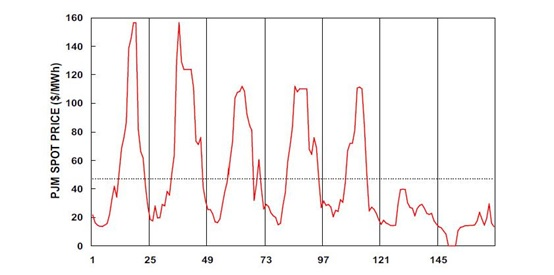
\includegraphics[scale=0.9]{figures/fig2-1.jpg}
	\centering
	\caption{Διακύμανση τις τιμής της ηλεκτρικής ενέργειας}
	\label{dataconnection}
\end{figure}

\subsection{Τίτλος Υπο-ενότητας}

\subsection{Τίτλος Υπο-ενότητας}

\subsection{Τίτλος Υπο-ενότητας}

κλπ.



